\documentclass[a4paper,12pt]{report}
\usepackage{fixltx2e}
\usepackage[english,frenchb]{babel}
\usepackage[utf8]{inputenc}
\usepackage[T1]{fontenc}
\usepackage{helvet}
\renewcommand{\familydefault}{\sfdefault}


\usepackage{float}
\usepackage{graphicx}
\usepackage{wrapfig}
\usepackage{subcaption}

\usepackage[chapter]{algorithm}
\usepackage{algorithmic}
\algsetup{linenodelimiter=}
\renewcommand{\algorithmiccomment}[1]{\##1}

\usepackage{amsmath}

\usepackage{perpage}
\MakePerPage{footnote}
\pagestyle{headings}

\usepackage[title,titletoc]{appendix}
\newcommand{\appsec}[1]{\newpage \section{#1}}
%syntax is:
%\begin{subappendices}
%  \appsec{appendix title}
%\end{subappendices}

\bibliographystyle{alphaurl}

\newcommand{\HRule}{\rule{\linewidth}{0.5mm}}


\title{Robot en essaim: explorez}
\author{Sacha Alcalde Mangen, Shankar Baba, Rosine Desmet, Nathan Dwek, Bernard Gonda}

\begin{document}

\begin{titlepage}
\begin{center}

% Upper part of the page. The '~' is needed because \\
% only works if a paragraph has started.

\includegraphics[width=0.4\textwidth]{EPB.jpg}~\\[1cm]

\textsc{\LARGE Ecole Polytechnique de Bruxelles\\Université Libre de Bruxelles}\\[1.5cm]

\textsc{\Large Rapport du projet de Ba2: Groupe 9}\\[0.5cm]

% Title
\HRule \\[0.4cm]
{ \huge \bfseries Robots en Essaim: Explorez\\[0.4cm] }

\HRule \\[1.5cm]

% Author and supervisor
\begin{minipage}{0.4\textwidth}
\begin{flushleft} \large
\emph{Etudiants:}\\
Sacha \textsc{Alcalde Mangen}\\
Shankar \textsc{Baba}\\
Rosine \textsc{Desmet}\\
Nathan \textsc{Dwek}\\
Bernard \textsc{Gonda}\\
\end{flushleft}
\end{minipage}
\begin{minipage}{0.4\textwidth}
\begin{flushright} \large
\emph{Superviseur:} \\
Ir. Anh Vu \textsc{Doan Nguyen}
\end{flushright}
\end{minipage}

\vfill

% Bottom of the page
{\large \today}

\end{center}
\end{titlepage}

\selectlanguage{english}
\begin{abstract}
The goal of this project was to design a swarm-intelligent behaviour for virtual robots using the ARGoS software. These robots had to explore an unknown environment with obstacles in order to ultimately loop between spots marked on the ground and a starting area. The fundamental paradigm was that a single set of rules would be followed independently by every robot, which would allow a swarm-intelligent behaviour to emerge through the robot interactions prescribed by these rules. For that to work, exploration, shortest path-finding and obstacle-avoidance algorithms were needed, along with elementary automated decision making, communication and odometry. These concepts were implemented using the ARGoS loop approach, which means that the same sequence of actions takes place at every step, while only events occurring during that step can influence these actions. However, a Dijkstra path-finding algorithm, which would only execute once before every trip while always providing the shortest trajectory, was also considered. A first working solution was produced using the Lua language, then put to the test and could quickly be enhanced accordingly thanks to the flexible framework. This allowed robots to loop between a starting area and spots of known position while avoiding collisions, and information was gathered on parameters meaningful for the experiment. Future development should be focused on optimizing these parameters and enabling robots to explore a fully unknown environment.
\end{abstract}

\selectlanguage{frenchb}
\begin{abstract}
Le but de ce projet était de créer une intelligence en essaim pour des robots modélisés dans le simulateur ARGoS. Ceux-ci devaient explorer un environnement inconnu qui comportait des obstacles afin d'ensuite faire des allers-retours entre des zones marquées aux sols et leur nid de départ. Le principe de base était que le même ensemble de règles devrait être suivi de manière indépendante par chaque robot; la caractéristique intelligente de l'ensemble de robots devant émerger à travers les interactions entre robots prescrites par ces règles. Pour cela, des procédures d'exploration, de recherche du plus court chemin et d'évitement furent nécessaires ainsi que des principes de base de prise de décision, d'odométrie et de communication. Ces concepts furent mis en pratique en utilisant l'approche loop d'ARGoS, qui implique que le robot exécute la même séquence d'opérations à chaque pas. Cependant, une recherche du plus court chemin Dijkstra, qui ne serait faite qu'une seule fois avant chaque trajet d'un robot, tout en trouvant toujours le chemin le plus court, fut aussi considéré. Une première solution fonctionnelle en Lua fut construite, testée et ensuite améliorée en conséquence grâce au turnaround loop très court offert par ARGoS. Cette solution permet aujourd'hui au robot de faire des allers-retours entre leur nid et une ou plusieurs ressources dont ils connaissent la position à l'avance, tout en évitant les collisions dans un environnement inconnu. De plus, des informations ont été collectées sur des paramètres influençant l'expérience. La deuxième partie du quadrimestre devrait être consacrée à l'optimisation de cette solution et à permettre au robot d'explorer un environnement afin de trouver la position des sources à exploiter. 
\end{abstract}

\tableofcontents

\chapter{Introduction}

Le but du projet est d'établir un comportement en essaim à des robots afin qu'ils puissent explorer un environnement non connu à l'avance, et naviguer entre un nid et une ressource, qu'ils exploiteront \cite{cahierCharges}. Le nid sera représenté par une zone peinte au sol et les ressources par une lumière dans l'arène. Le nid sera la zone où les robots pourront recharger leur batterie. Effectivement, le fait que les robots possèdent une batterie, limitée à un aller-retour du centre à l’extrémité de l'arène, devra également être pris en compte. Des obstacles seront également présents dans l'arène. Les robots devront donc également être capable d'éviter tout type d'obstacles. ARGoS, un simulateur développé par le laboratoire IRIDIA, sera utilisé afin de simuler le comportement des robots dans l'arène.

\section{Intérêt du projet}

L'intérêt principal du projet est la compréhension du fonctionnement d'un comportement en essaim. La conception d'un comportement en essaim performant permettrait de remplacer les êtres humains par des robots dans des tâches dangereuses et où l'utilisation de ceux-ci serait trop coûteuse. Par exemple, l'exploration de la surface terrestre de Mars peut se faire à l'aide d'un essaim de robots ce qui enlèverait les problématiques de l'envoie et du rapatriement des astronautes à la fin de leur mission.

\section{Résultat attendus}

L'objectif premier est de trouver un comportement qui permet aux robots de survivre et d'exploiter une ressource de manière autonome dans un environnement non connu à l'avance.

Dans un premier temps, les robots seront considérés comme omniscient et connaîtront l'environnement à explorer. Dans un second temps, la comportement en essaim devra prendre en compte la non connaissance de l'environnement à explorer et inclura, donc, une mémoire permettant de stocker les données qui s'accumuleront. Une communication entre les robots pourra être envisagée par la suite.
Même si la tâche à accomplir est au niveau de l'essaim, ce dernier ne sera jamais programmé directement. Il devra être fait au travers du comportement individuel des robots. Des interactions locales entre robots, physiques ou non, émergera un comportement global qui devra être étudié et être rendu prévisible.

Des outils de mesure, afin de calculer la qualité du comportement en essaim, devront être élaborés. Ils devront établir la performance des solutions proposées en fonction des objectifs initiaux.

Pour résoudre la problématique donnée, le projet a été décomposé en trois grandes parties: l'intelligence artificielle, la trajectoire des robots et la prise de décision. 

\chapter{L'intelligence artificielle\label{chap:AI}}

Afin de mener à bien l'objectif énoncé dans l'introduction, les robots doivent se comporter de manière intelligente. Le plus important est l'interaction avec l'environnement. En effet, le choix de la bonne action est cruciale. Il est cependant délicat de définir qu'une seule bonne action. Ceci est développé plus bas, en introduisant un «nouveau concept» qui est la rationalité. 
De manière générale, un robot peut être assimilé à un agent qui reçoit des «percepts» par l'intermédiaire de ses capteurs. L'agent réagit alors en exerçant une action sur l'environnement grâce à ses effecteurs.
\begin{figure}[h!]
  \centering
  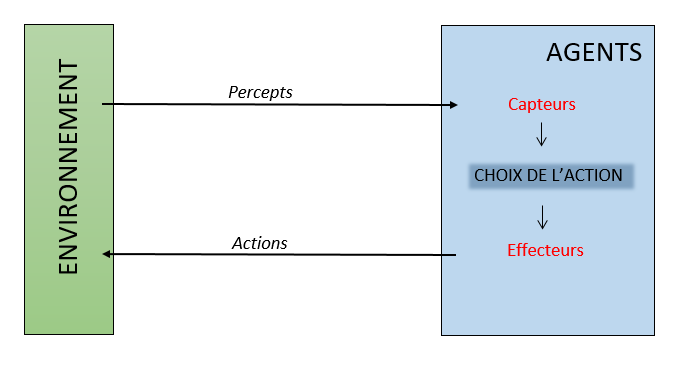
\includegraphics[width=0.7\textwidth]{cycleInteractionAI.png}
    \caption{Cycle d'interaction entre l'environnement et les agents}
\end{figure}
La description des différents capteurs et effecteurs du robot est faite ci-dessous dans le chapitre \ref{chap:argosFootbot}.

Comme énoncé précédemment la rationalité d'un agent peut être délicate à mesurer. D'après \cite{AIBrique}:
\begin{quote}
  \og{}La rationalité n'est pas synonyme de perfection, la rationalité maximise la performance espérée tandis que la perfection maximise la performance réelle.\fg{}
\end{quote}


En effet, dans un groupe composé de plusieurs agents, un choix d'action peut s'avérer bénéfique pour un agent mais mauvais pour l'ensemble du groupe. C'est pourquoi il est préférable de concevoir les mesures de performance en fonction de ce que l'on souhaite obtenir dans l'environnement et non en fonction de la façon dont devrait se comporter un agent.

A partir de cela, tout problème peut être formellement défini par cinq composantes. Tout d'abord l'état initial dans lequel commence l'agent, puis la description de ses différentes actions, c'est à dire toutes les actions possibles dans un état donné. Ensuite, vient le modèle de transition, il décrit ce que chaque action réalise. Ces trois premières composantes définissent l'espace des états du système, c'est à dire l'ensemble de tous les états accessibles par une séquence d'action à partir de l'état initial.

Dès lors l'espace d'état peut être interprété sous forme d'arbre où les nœuds représentent des états et les branches des séquences d'action. Il en découle la notion de chemin représentant une séquence d'états reliés par une séquence d'action.

La quatrième composante correspond au test but. Celle-ci détermine si un état donné est un état but. Enfin vient la cinquième et dernière composante, le coût du chemin. Elle permet d'attribuer une valeur numérique à un chemin en accord avec la mesure de performance imposée.
Maintenant qu'une présentation générale de l'intelligence artificielle a été faite, le comportement d'essaim d'agents intelligents peut être étudié. Pour ce faire, il s'est avéré très intéressant d'en comprendre le comportement à partir d'exemples se trouvant dans la nature. Les fourmis et les abeilles illustrent bien cela. Deux algorithmes mettant en avant leur comportement ont été développé ci-dessous.

\section{Algorithme des fourmis}

Cet algorithme est basé sur le comportement des fourmis dont une des particularités est la communication au travers de l'environnement par dépôts de phéromones.

L'algorithme se présente de la manière suivante. Pour commencer, une exploration de l'environnement est faite par les fourmis. Si l'une d'entre elles trouve une source, elle déposera, lors de son retour au nid, des phéromones tout au long du chemin qu'elle emprunte. Dès lors, lorsque que d'autres fourmis partiront à la recherche de nourriture, elles auront tendance à suivre le chemin  marqué de phéromones. Et à leur retour à la colonie, elles renforceront cette piste \cite{wikiFourmi}.

Cet algorithme illustre une communication indirecte d'un essaim et la manière dont ce dernier est influencé \cite{communicationFourmis}. L'autre algorithme, illustrant le comportement d'une structure organisée, est l'algorithme des abeilles.

\section{Algorithme des abeilles}

L'algorithme des abeilles est un «algorithme d'optimisation basée sur un comportement intelligent particulier des essaims d'abeilles».CITATION?

Dans cet algorithme, tout comme dans celui des fourmis, les abeilles explorent le milieu environnant le nid. Par contre, ces dernières partagent des informations de manière directe. En effet, si une source est trouvée, celle-ci débutera une danse qui aura pour but d'avertir les autres abeilles. Plus la source sera importante, plus la danse sera complexe.SOURCE

Comme observé dans ces algorithmes, la communication est indispensable à une bonne organisation d'un collectif d'individus. Dans le cadre de ce projet, le moyen dont les robots vont se partager les informations peut s'y inspirer.

D'une part, en s'inspirant de la communication des abeilles, les robots pourraient communiquer l'emplacement des sources de manière directe. Pour cela, celles-ci allumeraient leur LED pour communiquer l'emplacement d'une ressource. Ou d'autre part, pour communiquer indirectement, les robots pourraient déplacer les objets à l'aide de ses effecteurs. Par exemple, ils déplaceraient les obstacles dans son environnement de telle manière à créer un chemin qui mènerait du nid à la source.

Le prise en charge de la communication des robots ne sera traitée qu'au second quadrimestre. Mais tout ceci est concevable car les robots disposent d'effecteurs capables d'interagir sur l'environnement et de capteurs capables de cerner les différentes modifications de ce dernier.

\chapter[ARGoS et les footbots]{Présentation du simulateur ARGoS et des footbots\label{chap:argosFootbot}}

Dans le projet, on a à notre disposition des robots bien spécifiques (figure se trouvant ci-dessous). Ceux-ci possèdent des capteurs (des caméras, senseurs, scanners) et des effecteurs (des roues motrices, une balise et une pince). Les capteurs leurs permettent de recevoir des informations émanant de l'environnement et les effecteurs leurs donnent la possibilité d’interagir avec cet environnement.
\begin{figure}[h!]
   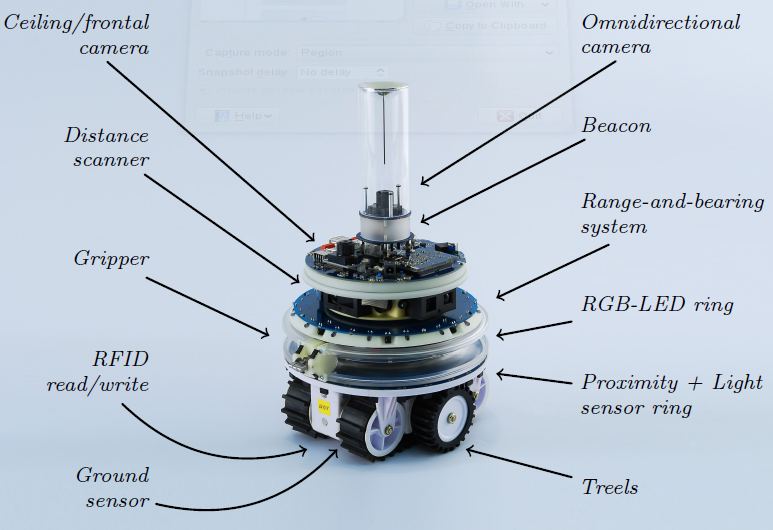
\includegraphics[width=\textwidth]{footbot.png}
      \caption{Les différents senseurs et actuateurs d'un footbot \cite{argosSite1}}
\end{figure}

Le comportement en essaim des robots devra être simulé dans ARGoS. Ce dernier est un simulateur de robots open source qui a initialement été développé au sein du projet Swarmanoid. Pour l'exécuter, un fichier XML est nécessaire. Il permet la configuration du programme pour une expérience spécifique. Pour dicter la conduite que doivent suivre les robots, un script est nécessaire. Ce script peut être écrit dans deux langages que gère ARGoS: C++ et Lua.

Vu que le script peut être écrit en Lua ou en C++, un choix entre ces deux langues doit être établi. Pour le bien du projet, il faut savoir optimiser le programme sans tomber dans un perfectionnisme inutile. On doit donc établir les avantages et inconvénients que possèdent ces deux langages tout en conservant en tête ce que requiert réellement le projet.

\chapter{Choix du langage informatique}

Lors de la présentation du simulateur ARGoS, deux choix de langage de programmation étaient possibles pour programmer les robots: C++ et Lua.

Après s’être familiarisé avec ces langages, la décision s'est portée sur Lua pour diverses raisons.

D'une part, les principaux avantages de C++, notamment, sa rapidité d’exécution et ses grandes librairies, ne semblaient pas primordiaux dans le cadre de ce projet. À cela s'ajoute les difficultés que ce langage aurait introduites. Plus spécifiquement, de meilleures connaissance aurait été nécessaire pour programmer, sans compter le temps perdu dans les débuguage du code.
D'autre part, Lua est proche du langage Python. Ce dernier a été étudié en BA1 à l'école polytechnique de Bruxelles. Comme Lua est un langage de scripting, il était plus adapté aux besoins du groupe grâce à sa facilité de concevoir des prototypes de programmes rapidement. Sa simplicité de compréhension a aussi favorisé une plus grande clarté du code des autres membres, ce qui a permis de dédier plus de temps à l’avancement du projet \cite{compC++,compLua}.

Il faut aussi souligner le fait que la nouvelle version d'ARGoS permet de compiler un fichier Lua en un seul clic grâce au compilateur intégré à ARGoS. Pour compiler un fichier C++, il faut passer par le terminal et appeler le compilateur pour ensuite exécuter le fichier compilé dans ARGoS. Cette étape supplémentaire peut être néfaste à la productivité sachant que l'on requiert souvent de tester le code qui a été écrit. Cette nouvelle version possède aussi, par défaut, un contrôleur Lua qui associe les différents capteurs à des fonctions de base exploitable dans un code Lua. Sur les quatre fonctions prédéfinies de LUA combiné a ARGoS (init, step, reset et destroy), les trois premières sont primordiales pour qu'ARGoS fonctionne. En effet ces fonctions s’exécutent une à une sur un seul robot puis l'autre et ainsi de suite. En C++, il aurait fallu réaliser cette étape en plus et même changer l'implémentation des fonctions de base.

Au vu des raisons énoncées ci-dessus, Lua a été choisi comme langage de programmation. 

\chapter{Trajectoire}

\section{Déplacement élémentaire}

Comme il a été présenté dans l'introduction sur l'intelligence artificielle, et vu en pratique dans la structure de base d'un comportement Lua interprétable par ARGoS, un footbot exécute à chaque step une séquence d'opérations. On peut distinguer dans cette séquence trois types d'opérations (cf chapitre \ref{chap:AI}): l'écoute des capteurs, la prise de décision et les interactions sur l'environnement par l'intermédiaire des effecteurs, que l'on nommera ici simplement sous le nom d'actions. Ces actions sont donc limitées et déterminées par les effecteurs dont dispose le robot et qui sont décrits au chapitre \ref{chap:argosFootbot}. Dans ce chapitre-ci, l'un des effecteurs primordiaux d'un footbot sera examiné: son déplacement.

Tout d'abord il est intéressant de se pencher sur le lien entre les paramètres physiques du robot et la manière dont celui-ci peut effectuer l'action simple «se rendre d'un point A à un point B» dans le cas où le robot agit seul dans un environnement sans obstacles. Ensuite, nous verrons comment le robot peut s’accommoder des obstacles (fixes, prévisibles) et autres robots (mobiles, imprévisibles) à partir d'une ou plusieurs de ces actions simples.

\begin{wrapfigure}{r}{0.17\textwidth}
  \vspace{-30pt}
  \begin{center}
    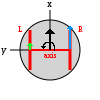
\includegraphics[width=0.15\textwidth]{robotWheels.png}
  \end{center}
  \caption{Signification physique de \(v_r,\: v_l,\: v_g \; et \; \omega_g \) \cite{argosSite1}}
\end{wrapfigure}
L'effecteur dont un footbot dispose afin de se déplacer est une paire de roues dont les vitesses peuvent être fixées de manière indépendante. A chaque instant, les seuls deux mouvements auxquels peut accéder le robot sont donc une translation parallèle aux roues et une rotation autour d'un point au milieu de l'axe des roues. La mécanique \cite{meca} nous indique que la composition de ces deux mouvements est suffisante pour permettre au robot de se déplacer librement dans un plan mais surtout, elle nous donne la relation entre les vitesses des deux roues et la vitesse générale ainsi que la vitesse de rotation du robot:
\begin{equation}
\begin{cases}
v_g=\frac{v_r+v_l}{2}\\
\omega_g=\frac{v_r-v_l}{l_{axe}}
\end{cases}  
\end{equation}

A partir de cette loi des vitesses, il est aisé de construire un algorithme permettant à un robot de converger vers sont but selon une trajectoire souple et à vitesse constante.
\begin{algorithm}                    
\caption{Convergence with no obstacle avoidance}
\label{simpleConvergence}
\begin{algorithmic}[1]
  \REQUIRE \(SPEED :=\) Fixed speed of the footbot \(> 0\)\\goal in arena
  \ENSURE footbot converges towards the goal at speed \(SPEED\)
  \WHILE{goal not reached}
    \STATE update footbot position and orientation
    \STATE \( \theta \leftarrow\) angle between the direction of the goal from the footbot and footbot orientation
    \STATE \( right\:velocity \leftarrow\) convergence(\(\theta,\:SPEED\))
    \STATE \( left\:velocity \leftarrow 2\cdot SPEED-right\:velocity\) \COMMENT{so that overall speed stays equal to SPEED}
    \STATE robot.wheels.set\_velocity(\(left\:velocity,\:right\:velocity\))
  \ENDWHILE
\end{algorithmic}
\end{algorithm}

Où convergence(\(\theta\), SPEED) fixe la convergence du robot vers son goal. Elle doit satisfaire:
\begin{equation}
  \begin{cases}
    convergence(0,SPEED)=SPEED\\
    convergence(\overset{\text{goal à gauche du robot}}{\overbrace{0<\theta\leq\pi}},SPEED)>SPEED\\
    convergence(\overset{\text{goal à droite du robot}}{\overbrace{0>\theta\geq-\pi}},SPEED)<SPEED
  \end{cases}
\end{equation}

Pour une fonction convergence(\(\theta, SPEED\)) donnée satisfaisant à cette condition (par exemple dépendance linéaire en \(\theta\)), le footbot peut donc se rendre d'un point A à un point B, tant qu'il ne rencontre pas d'obstacles sur son trajet. Notons que cet algorithme s'intègre particulièrement bien dans la fonction loop demandée par ARGoS. Dans notre projet nous avons choisi
\[convergence(\theta, SPEED)=(1+\kappa\frac{\theta}{\pi})SPEED\]
Où \(0< \kappa \leq 2 \) est un paramètre qui fixe l'intensité de la convergence.

\newpage
La manière la plus directe de permettre au robot d'éviter des obstacles quels qu'ils soient est d'exécuter une routine d'évitement à la place d'une routine de convergence lorsqu'un obstacle est détecté.
\begin{algorithm}                    
\caption{Convergence with obstacle avoidance}
\label{obstacleConvergence}
\begin{algorithmic}[1]
  \REQUIRE \(SPEED :=\) Fixed speed of the footbot \(> 0\)\\goal in arena
  \ENSURE footbot converges towards the goal at speed \(SPEED\) while avoiding obstacles
  \WHILE{goal not reached}
    \STATE update footbot position and orientation
    \STATE read proximity sensors \COMMENT{or whatever other sensor in use}
    \IF{no obstacles}
      \STATE \( \theta \leftarrow\) angle between the direction of the goal from the footbot and footbot orientation
      \STATE \( right\:velocity \leftarrow\) convergence(\(\theta,\:SPEED\))
    \ELSE
      \STATE \( right\:velocity \leftarrow\) avoidance(proximity sensor reading, \(SPEED\))
    \ENDIF
    \STATE \( left\:velocity \leftarrow 2\cdot SPEED-right\:velocity\) \COMMENT{so that overall speed stays equal to SPEED}
    \STATE robot.wheels.set\_velocity(\(left\:velocity,\:right\:velocity\))
  \ENDWHILE
\end{algorithmic}
\end{algorithm}

Où avoidance(proximity sensor reading) fixe la routine d'évitement du robot. Son implémentation est très libre et peut fortement varier en fonction du capteur utilisé pour détecter les obstacles. On peut par exemple utiliser le senseur proximity du footbot, qui associe à 24 directions autour du robot une valeur entre zéro et un: une valeur zéro indique qu'aucun obstacle n'est perçu dans la direction donnée tandis qu'une valeur supérieure indique qu'un objet a été détecté. Cette valeur augmente au fur et à mesure que le robot se rapproche de l'obstacle.\cite{argosSite1} Dans notre projet nous avons choisi
\[avoidance(dir, prox)=
  \begin{cases}
      \frac{-\alpha +(1-prox)^{\beta}\cdot dir}{11}SPEED & \text{si }dir \leq 12\\
      \frac{(22+\alpha )-(1-prox)^{\beta}\cdot (25-dir)}{11}SPEED & \text{si }dir \geq 12\\
  \end{cases}
\]
Où $ 1 \leq dir \leq 12 $ est la direction de l'obstacle perçu le plus proche et \hbox{$0 \leq prox \leq 1$} donne la proximité de cette obstacle. Comme présenté plus haut, ce sont les deux informations dont on dispose si l'on utilise le capteur de proximité.  \(1 \leq \alpha \leq 12 \) est un paramètre qui fixe l'influence de la direction de l'obstacle le plus proche et \(0 \leq \beta \) fixe l'influence de la proximité de cette obstacle. Cet évitement est partiellement tiré des exemples fourni sur le site du cours présentant ARGoS \cite{argosSite1}.

Grâce à cette routine d'évitement, ainsi qu'en utilisant l'algorithme présenté plus haut, il est déjà possible de produire une solution fonctionnelle à la partie déplacement du cahier des charges, même si on peut améliorer cette solution en fonction de la connaissance de son environnement dont dispose le robot.

Ainsi, dans le cas omniscient ou si le robot est capable de construire une carte de son environnement reprenant la position des différents obstacles il peut-être judicieux d'utiliser un algorithme de recherche du plus court chemin. La manière la plus directe de faire est de donner au footbot une liste de goal successifs qui le mèneront au goal final. Ceci  permet de réutiliser facilement les algorithmes déjà présentés tout en étant parfaitement compatible avec les valeurs de retour typiques d'un algorithme de recherche du plus court chemin. En effet, la plupart des recherches du plus court chemin utilisent une représentation en graphe d'un environnement. La valeur de retour d'une telle recherche est donc une liste des nœuds qu'il faut parcourir dans le graphe afin d'arriver au but final, ce qui est précisément ce que cet algorithme fait.
\begin{algorithm}                    
\caption{Convergence with path finding}
\label{pathConvergence}
\begin{algorithmic}[1]
  \REQUIRE \(SPEED :=\) Fixed speed of the footbot \(> 0\)\\intermediate goals list := list of points which lead to the goal while avoiding the obstacles\\goal in arena
  \ENSURE footbot converges towards the goal at speed \(SPEED\) while avoiding obstacles
  \FOR{intermediate goal in intermediate goals list}
  \WHILE{goal not reached}
    \STATE update footbot position and orientation
    \STATE read proximity sensors \COMMENT{or whatever other sensor in use}
    \IF{no obstacles}
      \STATE \( \theta \leftarrow\) angle between the direction of the goal from the footbot and footbot orientation
      \STATE \( right\:velocity \leftarrow\) convergence(\(\theta,\:SPEED\))
    \ELSE
      \STATE \( right\:velocity \leftarrow\) avoidance(proximity sensor reading, \(SPEED\))
    \ENDIF
    \STATE \( left\:velocity \leftarrow 2\cdot SPEED-right\:velocity\) \COMMENT{so that overall speed stays equal to SPEED}
    \STATE robot.wheels.set\_velocity(\(left\:velocity,\:right\:velocity\))
  \ENDWHILE
  \ENDFOR
\end{algorithmic}
\end{algorithm}

L'implémentation de l'algorithme de recherche du plus court chemin qui fournit intermediate goals list est un problème à part entière. Avant de l'examiner plus en détail, il faut noter que malgré l'utilisation d'une recherche du plus court chemin qui devrait a priori permettre d'éviter les obstacles, le test d'obstacles est toujours présent, ainsi que la possibilité d'évitement. Il est évident que ceci est fait pour permettre d'éviter des objets inattendus tels que d'autres robots, par exemple. Cependant, on peut dès lors se demander s'il ne faudrait pas aussi chercher de nouveau un plus court chemin après un évitement imprévu ou si le robot a dévié d'une distance significative de sa trajectoire prévue.

\section{Recherche du plus court chemin}

\subsection{Algorithme A* \cite{wikiA*}}

En informatique, A* est un algorithme informatique qui consiste à mettre en place un processus de traçage d'un chemin traversable efficace entre des points. Les points sont considérés comme des noeuds.

A* utilise une «best-first» recherche et trouve le chemin possédant le moindre coût à partir d'un nœud initial donné à un nœud but.

Pour cela, il utilise une fonction de coût pour déterminer l'ordre dans lequel les visites de recherche des nœuds de l'arbre vont s'effectuer. Cette fonction de coût est la somme de deux autres fonctions. La fonction coût de la trajectoire passée qui est la distance connue à partir du nœud de départ au dernier parcouru lors de la recherche. Et la fonction coût du chemin futur qui est une estimation heuristique de la distance entre le dernier nœud parcouru et le nouveau nœud à atteindre .

\begin{wrapfigure}{r}{0.3\textwidth}
  \vspace{-20pt}
  \begin{center}
    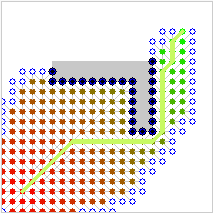
\includegraphics[width=0.28\textwidth]{aStar.png}
  \end{center}
  \caption{Représentation d'une éxécution de A*\cite{wikiA*}}
\end{wrapfigure}
Cet algorithme possède quand même des limites. Il est effectivement efficace dans le cas où l'on considère les robots comme omniscient, connaissant l'environnement et, donc, connaissant la position de la source et des obstacles se trouvant dans l'environnement. Dans le cas de non-omniscience, l'arène est inconnue et on ne possède aucunes données à propos de celles-ci. Et c'est ici que se trouve le plus grand défaut de l'algorithme A*.

A* détermine un chemin complet de nœuds pour arriver d'un noeud départ à un noeud but. Lorsqu'il ne possède pas de données complètes à propos de l'arène, il est bloqué lors de son exécution et ne peut donc pas déterminer le chemin que doit suivre le robot. Il faudra adapter l'algorithme A* afin de remédier à ce problème.

\subsection{Algoritme de Dijkstra \cite{wikiDijkstra}}

L’algorithme de Dijkstra est un algorithme servant à résoudre le problème du plus court chemin. Le principe de l'algorithme est le suivant:

Il s'agit de mettre en place progressivement un sous-graphe dans lequel sont classés les différents sommets. Un ordre croissant est établit entre les sommets et il est fixé en fonction de la distance minimale qui éloignent ces sommets à celui de départ. Cette distance correspond à la somme des nœuds parcourus.

Au début, les distances de chaque sommet par rapport au sommet de départ sont considérées comme infinie et on attribue à celui-ci une distance de 0.

Ensuite, au cours de chaque itération, les distances des sommets reliés par un nœud au dernier du sous-graphe sont mis à jour. Cette mis à jour consiste à ajouter la valeur du nœud à la distance séparant le sommet de départ à ce dernier sommet. Après cette mise à jour, l'ensemble des sommets, ne faisant pas partis du sous-graphe, sont examinés et celui qui possède la distance minimal y est ajouté.

Enfin, on répète l'exécution jusqu'à l'épuisement des sommets ou jusqu'à la sélection du sommet d'arrivée.
Voici 3 figures qui représentent un exemple du principe utilisé. Le but est de trouver le plus court chemin entre le point A et le point J. Comme dit précédemment, après chaque mise à jour, le sommet possédant la distance minimale est rajouté au sous graphe. La figure \ref{fig:dijkstra} représente bien cela.
\begin{figure}[h!]
        \centering
        \begin{subfigure}[h!]{0.4\textwidth}
                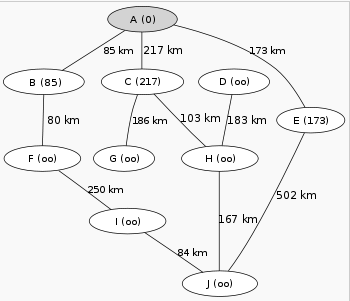
\includegraphics[width=\textwidth]{dijk1.png}
                \caption{Mise à jour initiale\\\(\;\)}
        \end{subfigure}   \begin{subfigure}[h!]{0.4\textwidth}
                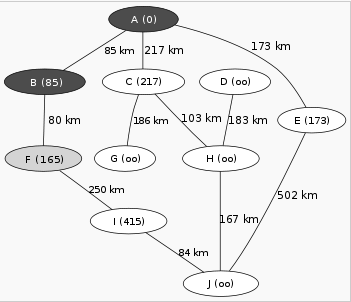
\includegraphics[width=\textwidth]{dijk2.png}
                \caption{Mise à jour et construction du sous-graphe}
        \end{subfigure}

        \begin{subfigure}[h!]{0.4\textwidth}
                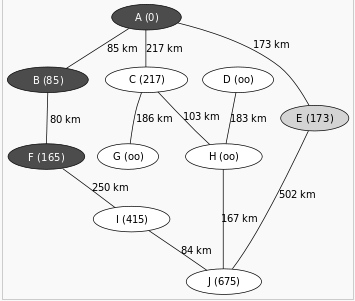
\includegraphics[width=\textwidth]{dijk3.png}
                \caption{Mise à jour et graphe final}
        \end{subfigure}
        \caption{\label{fig:dijkstra}Représentation d'une éxécution de Dijkstra \cite{wikiDijkstra}}
\end{figure}


En effet, le sommet E est rajouté au sous graphe et non le sommet I car la distance à parcourir entre A et E est plus petite que entre A et I.

Il faut souligner que cet algorithme possède le même inconvénient qu'A*. 

\chapter{Communication et prise de décision}

\section{Gestion de l'autonomie}
Une condition sur l'autonomie des robots a été imposée: l'autonomie est fixée dans le temps, ce qui signifie que leur batterie se décharge de manière constante à chaque pas d'ARGoS. Une valeur chiffrée n'a pas été imposée, mais les robots doivent juste être capables d'effectuer un aller-retour vers un point le plus éloigné de leur nid de départ à leur vitesse de régime. Une fois la batterie écoulée, le robot est rendu incapable de se déplacer mais pourra peut-être être dépanné par un autre membre de l'essaim dans le futur.

Puisque pour le moment le seul but d'un robot est d'exploiter une ressource, celui-ci peut avorter un aller retour dès qu'il estime qu'il n'est plus capable d'atteindre son but et de revenir ensuite à son nid.

\begin{algorithm}                    
\caption{Battery handling}
\label{algo:batterie}
\begin{algorithmic}[1]
  \REQUIRE \(0 \leq battery \leq 100 :=\) the battery left of the robot
  \ENSURE footbot tries to get back to nest when current goal judged not safely reachable
  \WHILE{goal not reached}
    \STATE update footbot position and battery
    \STATE \(cost \leftarrow evaluate\;cost(position,\;goal,\;[battery])\) \COMMENT{The cost of what is left to do}
    \IF{\(cost > battery\)}
      \STATE \(goal \leftarrow nest\) \COMMENT{Get back to the nest. If the footbot is already on its way back, this doesn't do anything. Appropriate to try to get to the nest when you know you don't have enough to get there?}
    \ENDIF
  \ENDWHILE
\end{algorithmic}
\end{algorithm}
Où evaluate cost(position, goal, [battery]) est la fonction qui évalue l'énergie nécessaire à l'accomplissement du reste du trajet. On peut par exemple utiliser la distance à vol d'oiseau restante à parcourir accompagnée d'un facteur de sécurité, ou alors utiliser une approche heuristique utilisant le rapport entre la batterie utilisée jusqu'au step courant et le déplacement net parcouru vers le but.

En vue de la prochaine étape (la non omniscience des robots), le choix d'implémentation de la batterie autorise des sacrifices, c'est à dire, si un robot, étant à une position, estime devoir aller à une autre position et si sa batterie le lui permet, il ira à cette nouvelle position, sans toutefois vérifier qu'en y allant il pourra rentrer à la base recharger sa batterie. Ce choix favorise l'exploration de l'arène en mettant en avant la réussite de l'ensemble du groupe et non la réussite personnelle, pouvant être interprété comme la recharge de la batterie. Cependant des modifications doivent encore être apportées car nous ne pouvons nous permettre de sacrifier l'ensemble des robots, faute de quoi l'objectif ne sera pas atteint.

\chapter{Résultats obtenus}

La première partie du projet consiste à installer ARGoS, guider un robot à un point donné et remplir l'objectif lorsque les robots sont omniscients comme le présente le cahier des charges \cite{cahierCharges}. Celle-ci a, en effet, été achevée. L'installation a été réalisée avec succès par tous les membres du groupe. Les robots parviennent aux points désignés tout en évitant les obstacles. De plus, ils peuvent, étant omniscients, faire des allers-retours entre le source et le nid. Les robots ont aussi la faculté de détecter une source grâce à ses senseurs et de tenir compte de l'épuisement de leur batterie. Ceci est illustré sur la figure \ref{fig:ourArgos}. Dans le cas de la figure \ref{fig:argosNest}, on  peut observer les robots qui se dirigent vers la source. Sur l'autre figure, les robots sont  de retour au nid.

\begin{figure}[h!]
        \centering
        \begin{subfigure}[h!]{0.4\textwidth}
                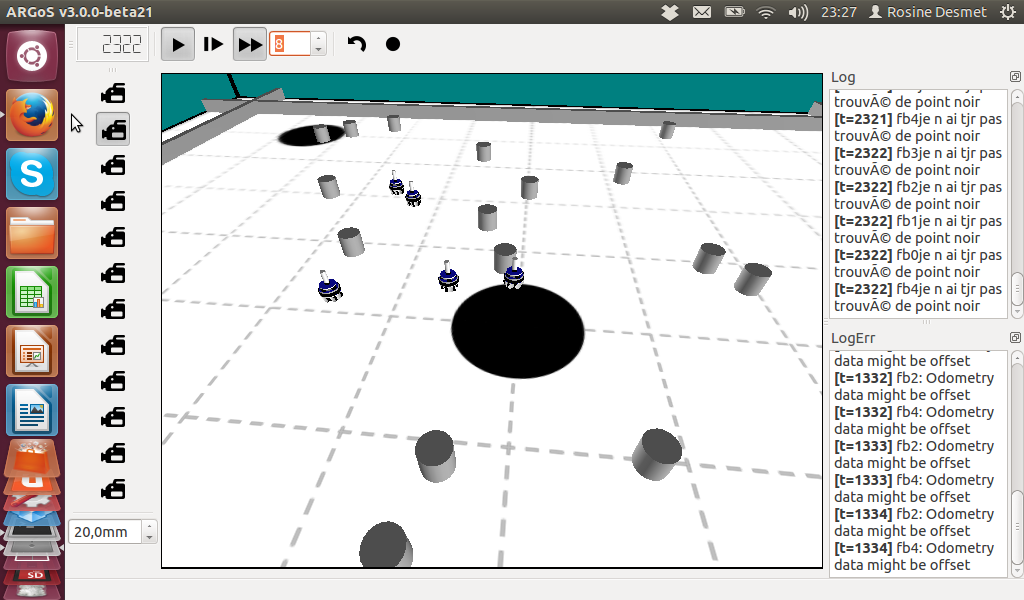
\includegraphics[trim = 60mm 40mm 75mm 45mm, clip, width=\textwidth]{ourArgos1.png}
                \caption{footbots allant à la source}
        \end{subfigure}   \begin{subfigure}[h!]{0.4\textwidth}
                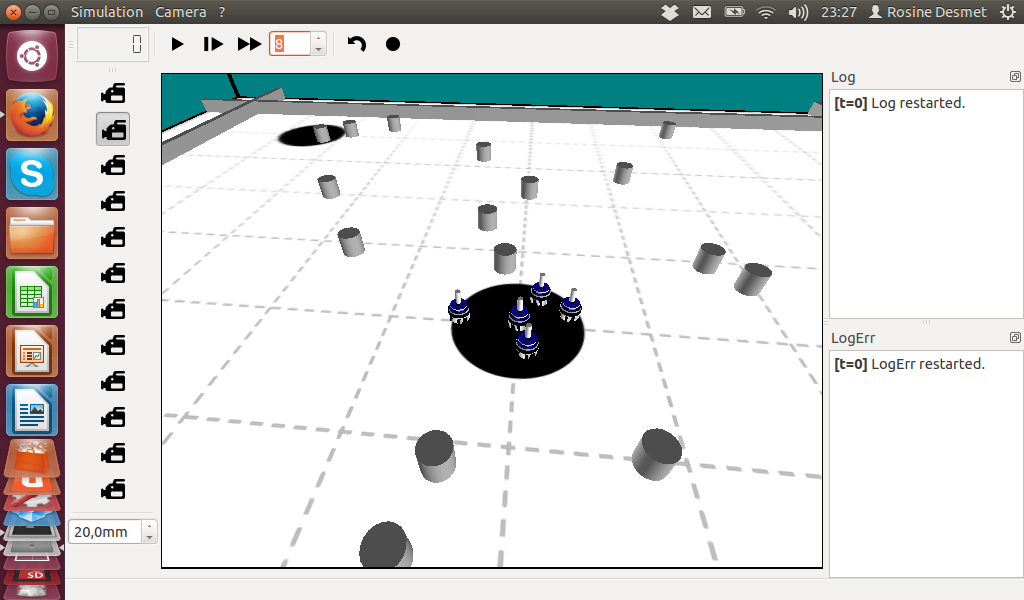
\includegraphics[trim = 60mm 40mm 75mm 45mm, clip, width=\textwidth]{ourArgos2.png}
                \caption{footbots dans le nid\label{fig:argosNest}}
        \end{subfigure}
        \caption{Exécution d'ARGoS avec le comportement produit\label{fig:ourArgos}}
\end{figure}

La création d'une collaboration au sein de l'essaim, le choix et l'intégration d'une communication entre robots, font partie de la seconde partie du projet. A ce niveau, grâce à une études des déplacements de base, la non-omniscience des robots peut déjà être gérée et des recherches sur la communication entre robots ont déjà été faites comme présenté au chapitre \ref{chap:AI}.

\chapter[Fonctionnement du groupe]{Fonctionnement du groupe \cite{bapp}}

\section{Général}

Le groupe est composé de 5 membres. Chaque membre a sa manière de travailler, de comprendre, de communiquer. Une des difficultés d'un travail d'équipe est de pouvoir combiner tous ces caractères pour que le projet se déroule dans les meilleures conditions et que chacun puisse trouver sa place. Donc pour comprendre le fonctionnement de chacun, chaque membre a dû présenter ses points forts et ses points faibles. Le but de cette démarche est de mettre en avant ses points forts et d'améliorer ses points faibles durant le projet. Des tensions sont tout de même survenues. En effet, le manque de communication a souvent mené de groupe à mal se coordonner.

\section{Organisation}

Le groupe se fixe une réunion par semaine. Les tâches à effectuer pour la prochaine réunion sont distribuées à la fin de celle-ci et notées dans les PV qui sont généralement envoyés dans les 48h. De rôles d'animateur et secrétaire sont réattribués toutes les 4 semaines. Pour diriger au mieux le projet, un diagramme de Gantt (cf.: annexe) a été conçu pour avoir une vision globale de l'avancé de celui-ci et également se fixer des dates butoirs.

\section{Communication}

Dans un premier temps, un groupe sur facebook a été créé. C'est un moyen simple et rapide de se communiquer les informations mais une communication par mail reste préférable. Pour le partage, des codes, des fichier et des sources des recherches, les dispositifs github, dropbox et zotero ont été mis en place. L'emploie de ces 3 dispositifs n'a pas encore été exploité au mieux mais son apprentissage est bénéfique non seulement dans le cadre de ce projet mais également pour plus tard. 

\chapter{Conclusion}

En conclusion, une compréhension de l'intelligence artificielle, du fonctionnement des robots et l'apprentissage de Lua ont permis d'atteindre les objectifs du 1er quadrimestre, ceux-ci étant de guidé les robots du nid à la source et de les programmer pour qu'ils puissent y faire des allers-retours. 
Les prochains objectifs à atteindre sont la mise en place d'un moyen de communication et d'exploration optimale l'environnement. Quelques options vont probablement être ajoutées dont l'introduction d'un système de priorité, dans le cas ou 2 robots cherchent à s'éviter, et une batterie se déchargeant de manière différente suivant l'état du robot (au repos ou en mouvement). De plus, une étude du comportement en essaim généré par notre code sera menée afin d'évaluer l'«intelligence de l'essaim».

\listofalgorithms

\addcontentsline{toc}{chapter}{Tables des algorithmes}

\listoffigures

\addcontentsline{toc}{chapter}{\listfigurename}

\nocite{*}

\bibliography{rapport}

\addcontentsline{toc}{chapter}{\bibname}

\end{document}          
